\section{The Large Hadron Collider}
\label{chp:det:LHC}

The LHC \cite{Evans:2008zzb} is a circular proton-proton collider located at the European Council for Nuclear Research (CERN). The machine is hosted in a 27 km circumference tunnel built between 50 m and 170 m underneath the French-Swiss countryside outside Geneva. Not only it is the world's largest collider but, with the current operation at a beam energy of 6.5 $\tev$ and its expected upgrade to the design energy of 7 $\tev$, it is also the most powerful.  It was designed to extend the reach of previous accelerators in the study of SM processes and searches for new phenomena.\par
The centre-of-mass energy increased by about a factor of seven with respect to the Tevatron collider at Fermilab \cite{fermilab}, while the high instantaneous luminosity (up to $10^{34}$ cm$^{-2}$s$^{-1}$) allows access to very rare processes and precision measurements. These considerations ultimately motivated the choice of a proton-proton collider. For protons the energy loss in a curved trajectory due to synchrotron radiation\footnote{The energy emission per turn is proportional to $(E/m)^{4}$, where $E$ and $m$ are the energy and mass of the particle respectively.}  is considerably smaller than for electrons and this allows accelerating protons more efficiently in a circular machine. At the same time, a hadron collider probes multiple energy scales simultaneously due to the momentum distribution of partons inside the protons.  A proton-antiproton collider alternative was rejected due to the difficulties of producing and operating high-intensity antiproton beams, which would have resulted in a lower peak luminosity. The LHC is also able to accelerate and collide lead ions at the nominal energy of 2.76 $\tev$/nucleon, for a total centre-of-mass energy of 1.15 $\pev$.

\subsection{CERN accelerator complex}

As for any other large particle collider, the energy of the colliding particles is gradually increased by subsequent acceleration steps; this solution has high flexibility and allows for a more efficient beam production. At the same time, intermediate accelerator machines provide beams that are used in other lower-energy experiments. A sequence of accelerators, shown in figure \ref{sec:det:fig:acccomplex}, is involved in the preacceleration of the protons before they are injected into the LHC ring \cite{Benedikt:2004wm}.

\bfig[h!]
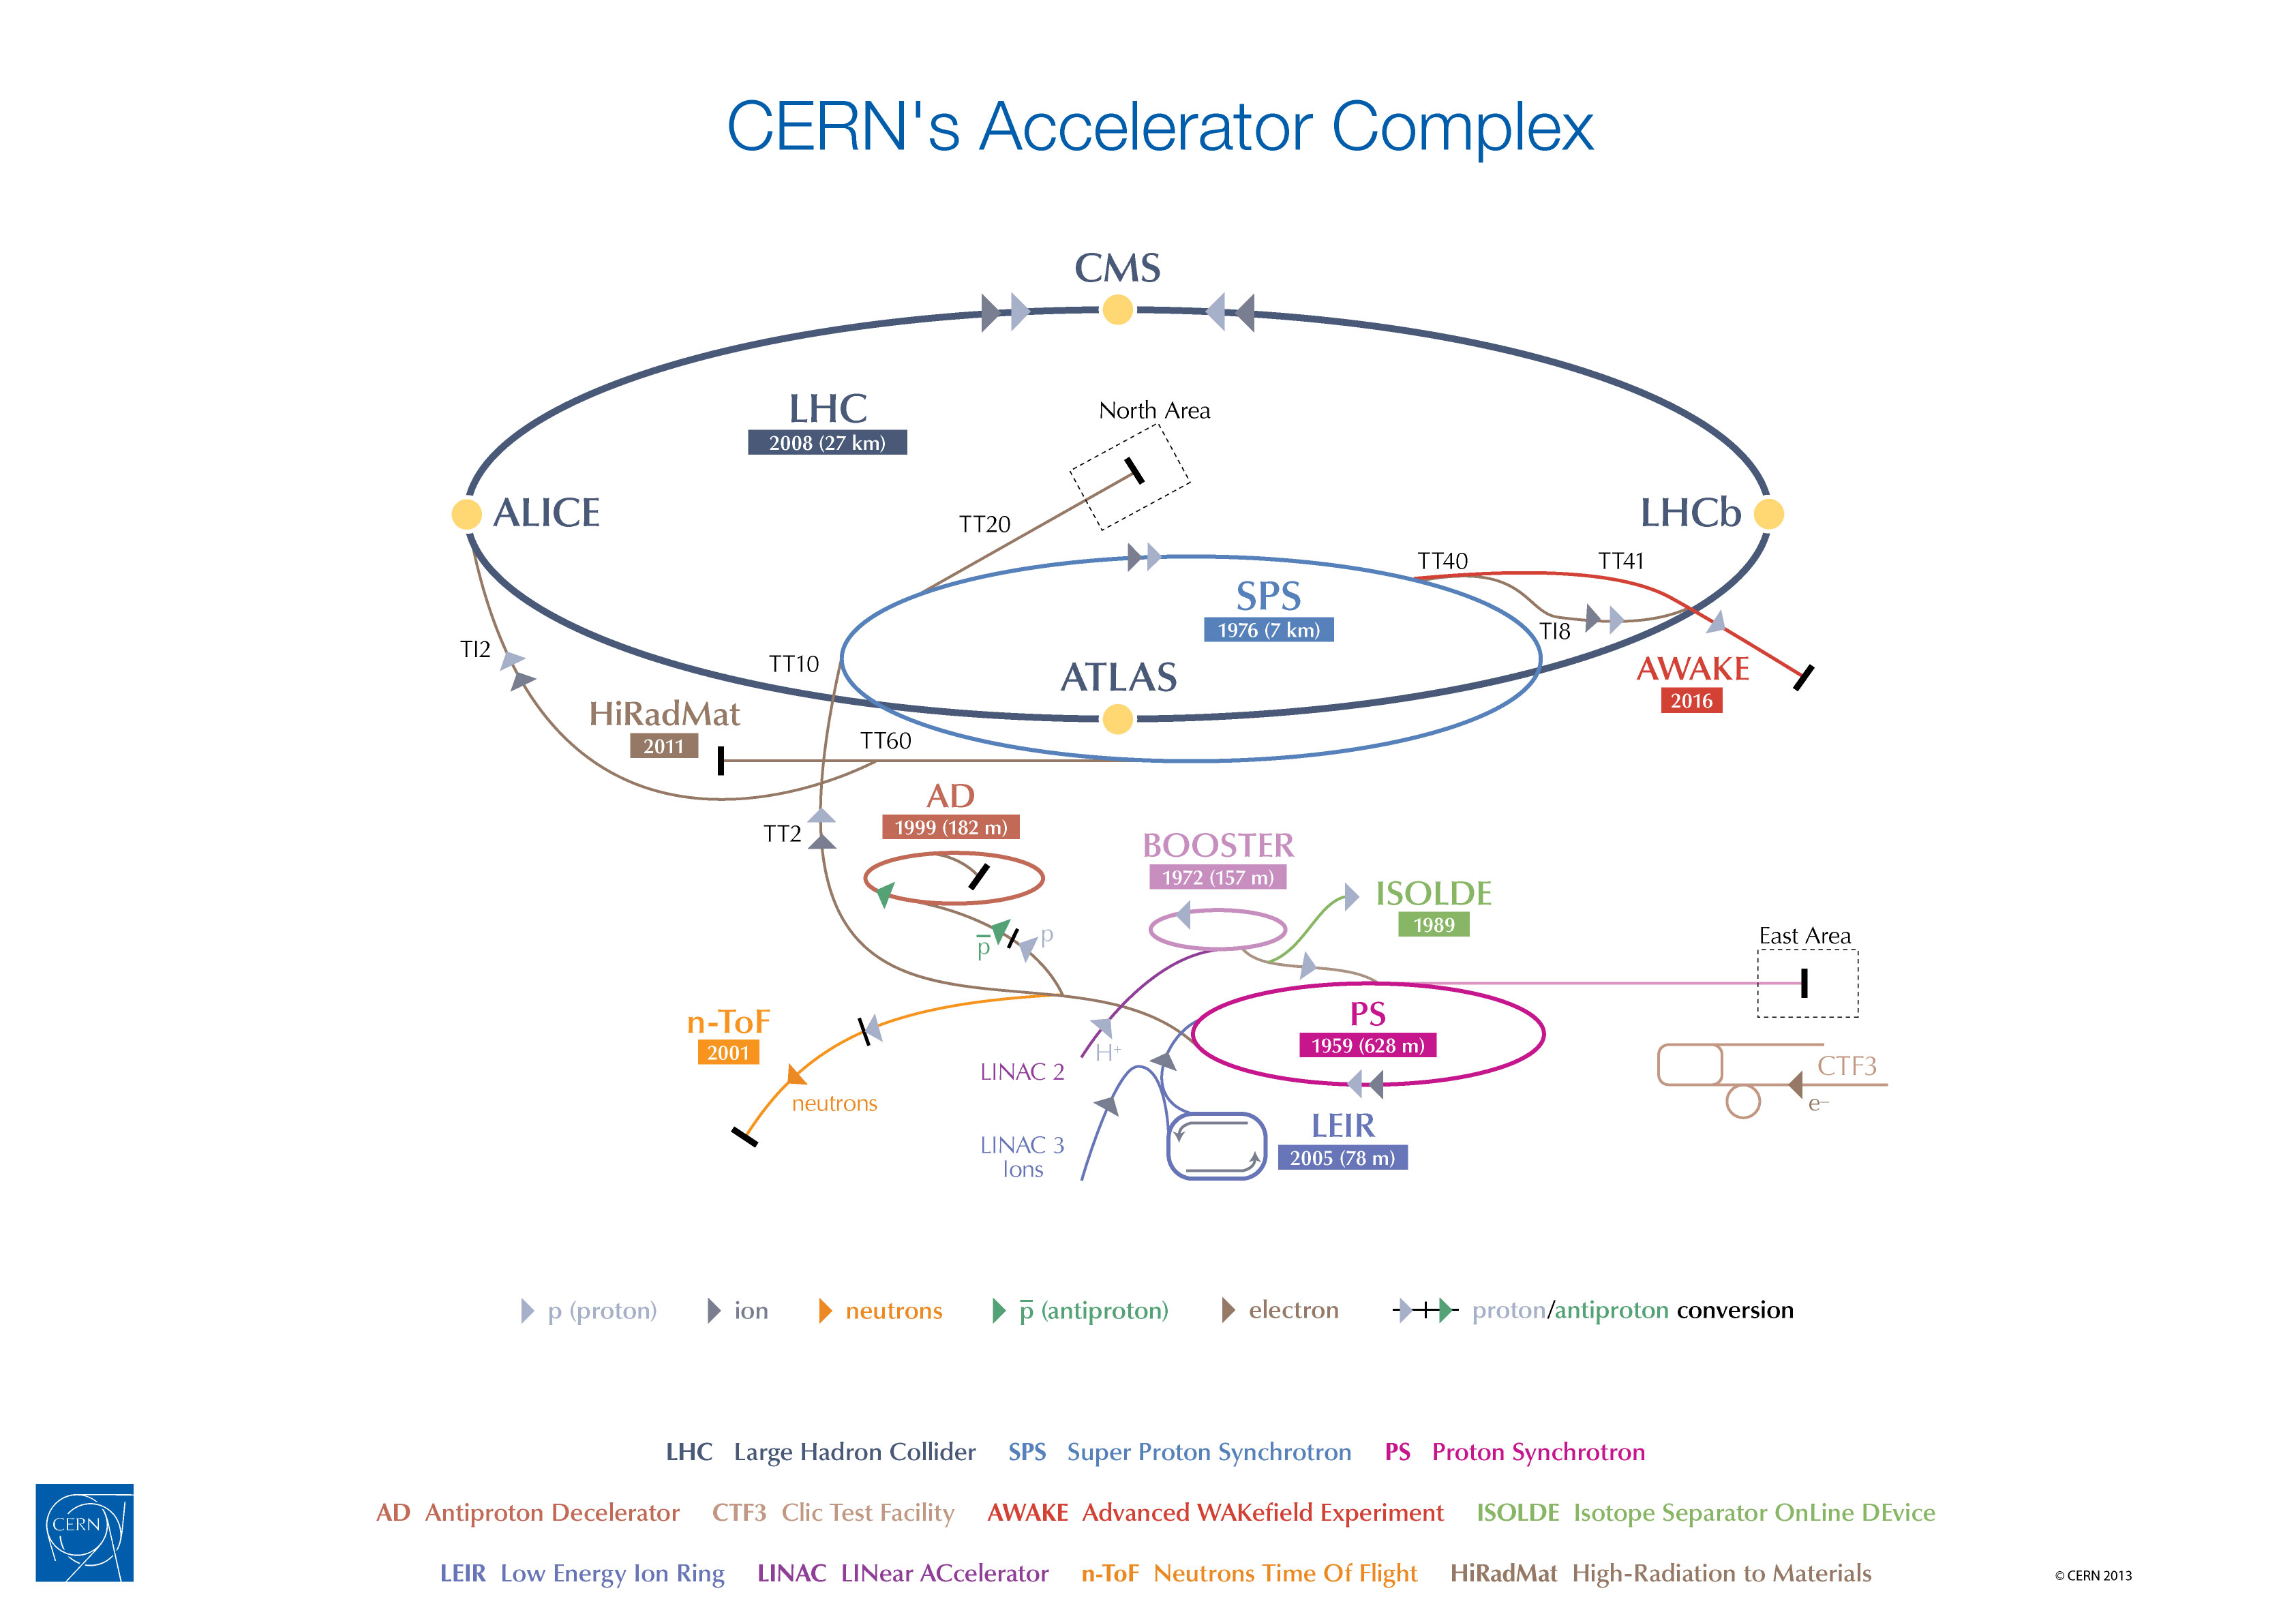
\includegraphics[width=\textwidth]{figures/Detector/CERNaccelerator}
\captionsetup{width=0.85\textwidth} \caption{\small Schematic view of the CERN accelerator complex. The four main LHC experiments are shown at the interaction points.}
\label{sec:det:fig:acccomplex}
\efig

Protons are obtained from hydrogen gas by breaking the molecules and stripping the electrons from hydrogen atoms. Protons are accelerated in the Linear Accelerator 2 (LINAC2) to 50 MeV and grouped into bunches. They are then transferred to the 157 m long Proton Synchrotron Booster (PSB), where they reach an energy of 1.4 $\gev$. After the PSB, protons are injected into the 628 m long Proton Synchrotron (PS), where their energy is ramped up to 25 $\gev$. In both the PSB and the PS protons are squeezed in very tight bunches that are the base bunch structure of the LHC. The last stage of preacceleration is done in the 7 km long Super Proton Synchrotron (SPS), where the protons are brought to an energy of 450 $\gev$ before injection into the LHC ring in two opposite directions. The connection between the LHC and the SPS is done through two 2.5 km long transfer lines.

\subsection{LHC design and machine parameters}
\label{chp:det:LHC:design}

One of the main contraints to reduce the cost of the LHC construction was the need to reuse the tunnel previously hosting the Large Electron Positron Collider (LEP).  The technological challenge of the LHC was the mass production of magnets necessary to maintain 7 $\tev$ protons in a circular trajectory with a radius of 4.3 km. A total of 1232 dipole magnets have been assembled in the LHC. Each magnet produces a bending field of up to 8.33 T thanks to superconducting coils made of niobium-titanium (NbTi) kept at a temperature of 1.9 K by superfluid helium. This makes the LHC the largest cryogenic system in the world. Each dipole contains two vacuum chambers in one single cryostat with magnetic fluxes that go in opposite directions, which allows the acceleration of two proton beams in opposite directions. This structure was needed to reduce the size of the cryostat and the cost of the cryogenic system.  The main acceleration from 450 $\gev$ to a maximum of 7 $\tev$  happens in the LHC with eight resonant Radio-Frequency (RF) cavities per beam. The electric field of those RF cavities oscillates at 400 MHz and increases the beam energy by 0.5 $\mev$/ turn. The field intensity at the maximum energy is around 5.5 MV/m.\\ \indent One of the important aspects in the design of an accelerator is the overall interaction rate that the LHC, in our case, can provide to the experiments.
The cross section, $\sigma$, describes the likelihood for a certain reaction -- the effective area that one particle presents to another particle for that reaction to occur. The instantaneous luminosity, $\lag(t)$, describes how frequently particles encounter each other, per unit of area and time. The overall interaction rate is equal to  $\sigma \times \lag(t)$. The total number of interactions for a certain process in a time interval [$t_{1}$,$t_{2}$], is given by:

\be
N_{\rm proc} = \int_{t_{1}}^{t_{2}} \sigma_{\rm proc} \times \lag(t) dt = \sigma_{\rm proc} \times \lag_{\rm int}(t_{1}, t_{2}),
\label{sec:det:eq:Nint}
\ee

\noindent where it is assumed that the cross section $\sigma_{\rm proc}$ does not depend on time and where $\lag_{\rm int}(t_{1}, t_{2})$ is the integrated luminosity for the time interval [$t_{1}$,$t_{2}$]. The requirement of high statistical accuracy of the data is translated into a requirement of high integrated luminosity of the accelerator. The instantaneous luminosity of the LHC at any Interaction Point (IP) depends on the beam bunch structure, the beam parameters and how well they can be controlled. For beams with equal parameters and approximately Gaussian spatial distributions, the instantaneous luminosity can be expressed as:

\be
\lag = N_{b} \cdot F\frac{n^{2}f_{\rm rev}}{4\pi \sigma_{xy}}, \,\, \sigma_{xy} = \sqrt{\frac{\epsilon\beta^{*}}{\gamma}},
\label{sec:det:eq:lumi}
\ee

\noindent where $N_{b}$ is the number of bunches present in each beam, $n$ is the number of protons in each bunch, $\sigma_{xy}$ is the transverse beam size at the IP, $f_{\rm rev}$ is the revolution frequencies of the bunches, $\gamma$ is the Lorentz factor, $\beta^{*}$ is the betatron function at the collision point, $\epsilon$ the normalised beam emittance, and $F$ is a geometric luminosity reduction factor that takes into account the beam crossing angle at the IP. 
The LHC beam parameters have been optimised to maximise the instantaneous luminosity at each IP taking into account various performance limitations and machine boundary conditions.\par
Due to the high frequency of collisions and the high density of the bunches necessary to achieve high luminosity, there is a non-zero probability that several events, originating from different $pp$ collisions, may occur simultaneously. These events are referred to as ``pileup'' and are categorised as in-time or out-of-time pileup. In-time pileup events are caused by additional $pp$ interactions in the same bunch crossing. The out-of-time pileup occurs when traces from an event in a different bunch crossing are recorded. The mean number of interactions per bunch crossing $\langle\mu\rangle$, which is taken as measure of the pileup activity, is shown in figure \ref{sec:det:fig:pileup}. The instantaneous luminosity is not constant over time, slowly degrading due to the bunch collisions, multiple Coulomb scattering within each bunch, and the scattering of protons against residual gas atoms inside the beam pipe. Therefore, the integrated luminosity depends on the luminosity lifetime, defined as the time that the beams are left orbiting in the LHC, and the beam turn-around time, defined as the time that passes between the beams being dumped and the beams being stable and ready for collisions again. More details about the LHC performance can be found in reference \cite{Bruning:2004ej}.

\bfig[h!]
\centering
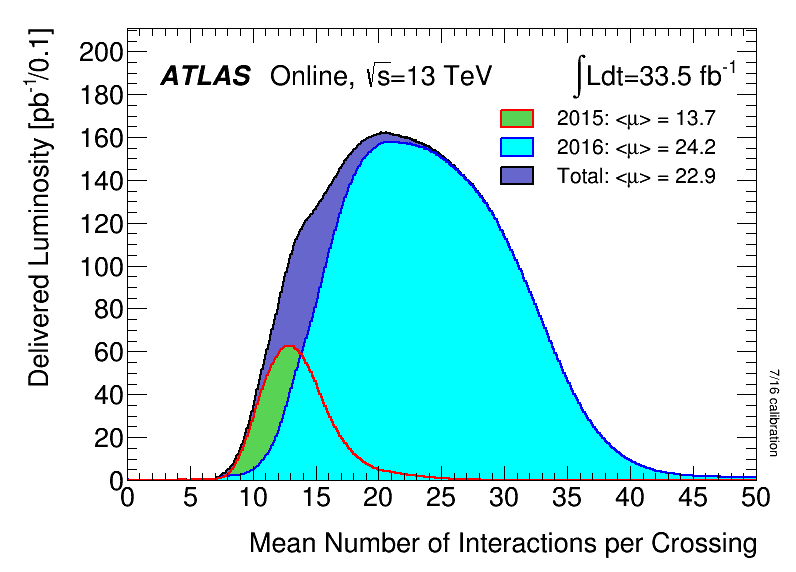
\includegraphics[width=0.5\textwidth]{figures/Detector/mu_2015_2016_LHCC.png}
\captionsetup{width=0.85\textwidth} \caption{\small Average number of interactions per beam crossing during the 2015 and 2016 LHC runs.}
\label{sec:det:fig:pileup}
\efig

\subsection{LHC experiments}

The LHC beams cross in four IPs, in each of which a particle detector is installed to record the collisions.  Earlier infrastructures, with some modifications to accommodate the LHC, were reused in order to further reduce the costs. Two of them are hosted in sites where before there were LEP experiments, while for the other two IPs new sites were needed. ATLAS \cite{ATLASjinst} and CMS \cite{CMS} are general-purpose experiments located at opposite IPs in the LHC ring. The independent design of the two experiments is of primary importance since it allows for cross-confirmation of measurements and possible new discoveries. LHCb \cite{LHCb} is a single-arm spectrometer designed to cover the forward region to perform dedicated studies of CP violation in $B$-meson decays and other studies of flavour physics, while ALICE \cite{ALICE} is designed to explore the formation of quark-gluon plasma in collisions of heavy ions. In addition to these four large experiments, three smaller experiments, LHCf \cite{LHCf}, TOTEM \cite{TOTEM} and MoEDAL \cite{MoEDAL}, are placed in the LHC ring. The LHCf experiment has been designed to study neutral hadrons emitted at low angles with respect to the beam pipe and it has been installed in the vicinity of ATLAS. CMS hosts TOTEM, which measures the total cross section through elastic and diffractive scattering of protons. The MoEDAL experiment is placed near LHCb and its purpose is the search for massive long-lived particles and magnetic monopoles.

\subsection{From first beam to world's record energy and luminosity}

After almost 15 years of prototyping the required technologies and an additional eight years of installation and commissioning of collider components, the LHC was officially completed and ready to start on the 10th of September 2008. Unfortunately, a serious accident occurred on the 19th of September, and the LHC operation had to be postponed and rescheduled. A faulty electrical connection
between two magnets ceased to be superconducting, causing mechanical failure of the cryogenic vessel followed by the leakage of around six tonnes of liquid helium. A total of 53 magnets were damaged and vacuum conditions in the beam pipe were lost. A total of 20 dipoles were replaced with spares, and new techniques to prevent a similar incident were developed. In December 2009 the LHC delivered first beams at a new world's record energy of 1.18 $\tev$. The new plan established that the LHC should provide proton beams of 3.5 $\tev$ during its initial operation from 2010 until 2012, and that it would be prepared to operate with proton beams of 7 $\tev$ only after a long shut-down period in 2013 and 2014.\par
In March 2010, Run 1 of the LHC started with the first collisions at a beam energy of 3.5 $\tev$, setting a new record for the energy achieved at a particle collider. The centre-of-mass energy was kept at 7 $\tev$ also during all of 2011. For the 2012 data taking the beam energy was increased to 4 $\tev$, for a center-of-mass energy of 8 $\tev$. In early 2010 the peak luminosity reached $2\times10^{32}$ cm$^{-2}$s$^{-1}$ obtained with $348$ colliding bunches of approximately $0.9 \times10^{11}$ protons each with a bunch spacing of 150 ns. In 2011 the peak luminosity reached $3.7\times 10^{33}$ cm$^{-2}$s$^{-1}$, increasing the number of bunches to 1380 with a minimum separation of 50 ns and the number of protons per bunch to $1.45 \times 10^{11}$. A further increase in luminosity was achieved by reducing the beam transverse size at the IP in order to increase the probability of $pp$ collisions per crossing. In 2012  a further reduction of the beam transverse size and an increase to the bunch intensity to 1.3 times the designed value allowed to reach a peak luminosity of $7.7\times10^{33}$ cm$^{-2}$s$^{-1}$. During the long shutdown (LS1), started on the 16th of February 2013, all electrical connections between superconducting magnets were consolidated allowing the LHC to reach higher energy and luminosity during Run 2. In figure \ref{sec:det:fig:consolidations} a summary of the LHC maintenance carried out during LS1 is shown.\par
In June 2015 LHC Run 2 started recording the first collisions at a beam energy of 6.5 $\tev$, setting a new record. During the year the number of bunches was increased up to 2244 with a minimum separation of 25 ns. For 2016 data taking the LHC achieved the current luminosity record for a hadron machine of $1.4 \times 10^{34}$ cm$^{-2}$s$^{-1}$  by further reducing the beam transverse size. Table \ref{sec:det:tab:LHCparam} shows the values of the beam parameters for the design operation, as well as those used during Run 1 and early Run 2 data taking.

\bfig[t!]
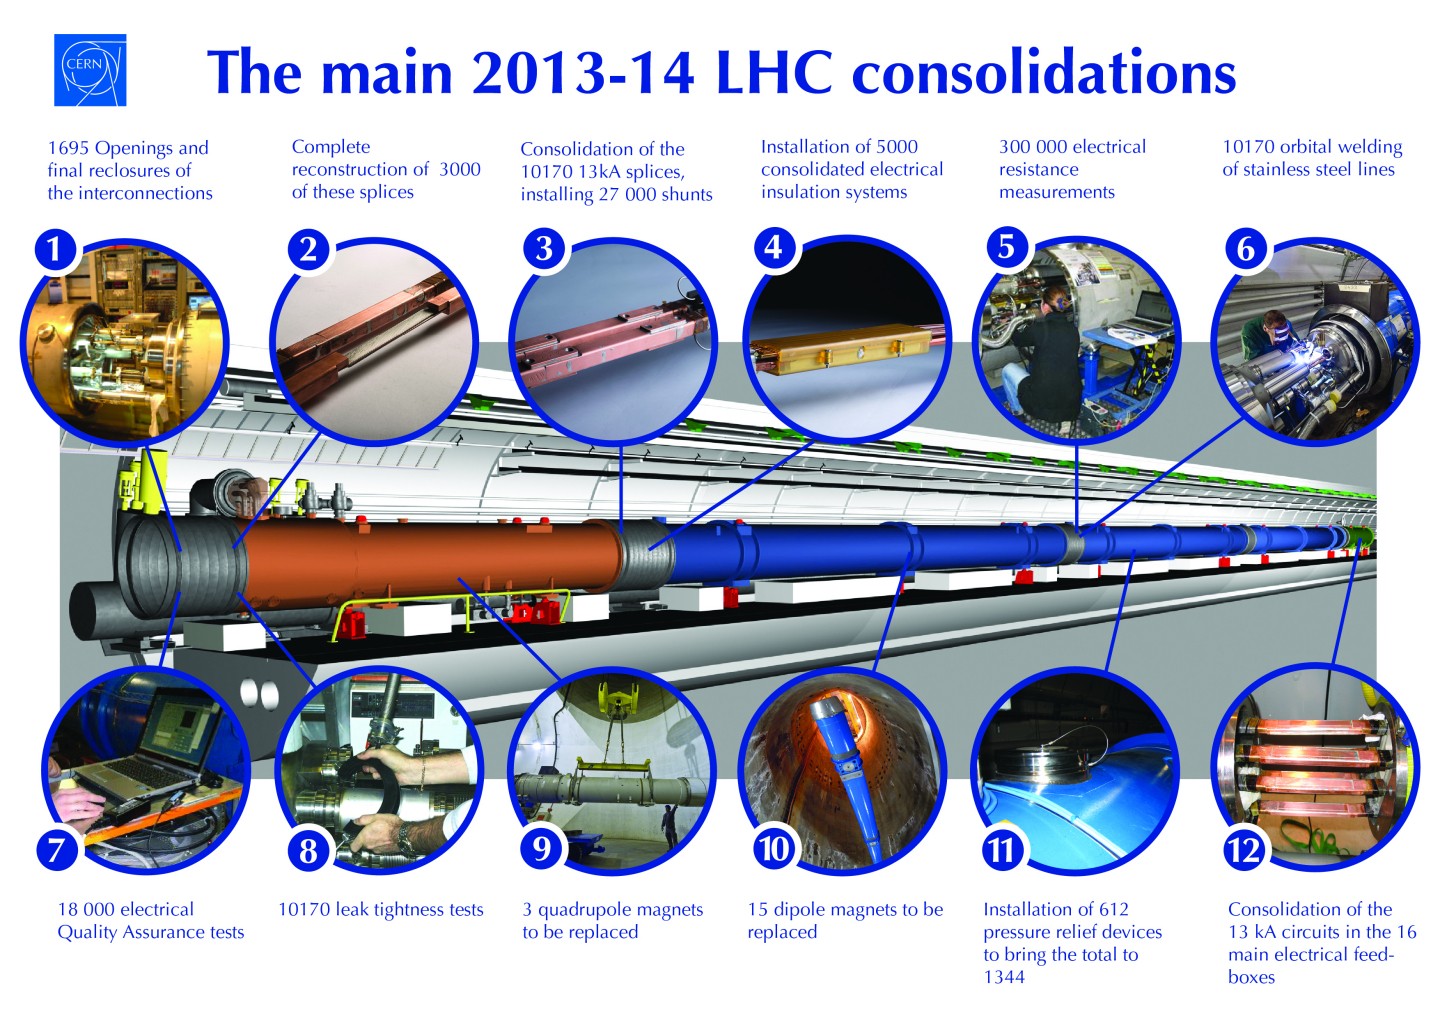
\includegraphics[width=\textwidth]{figures/Detector/LHCconsolidationsEng.jpg}
\captionsetup{width=0.85\textwidth} \caption{\small The main LHC consolidations during LS1.}
\label{sec:det:fig:consolidations}
\efig


\begin{table}
\footnotesize
\begin{center}
\begin{tabular}{c|c|c|c|c}
  \hline \hline
  Parameter & Design value & Run 1 & 2015 & 2016 \\
  \hline
  Beam energy ($\tev$) & 7 & 3.5--4 & 6.5 & 6.5 \\
  Beta function $\beta^{*}$ (m) & 0.55 & 1.5--0.6 & 0.8 & 0.4 \\
  Maximum num. bunches/beam & 2808 & 1380 & 2244 & 2220 \\
  Max. num. protons/bunch & $1.15\times10^{11}$ & $(1.45--1.7)\times10^{11}$ & $1.15\times10^{11}$ & $1.3\times10^{11}$\\ 
  Bunch spacing (ns) & 25 & 75--50 & 50--25 & 25 \\
  Peak luminosity (cm$^{-2}$s$^{-1}$ ) & $1\times10^{34}$  & $7.7\times10^{33}$  & $6\times10^{33}$  & $1.4\times10^{34}$  \\
  Emittance $\epsilon_{n} (\mu {\rm rad})$ & 3.75 & 2.5 & 2.5& 2.5 \\
 Max. $\langle\mu\rangle$ & 19 & 37 & 30 & 50 \\
  \hline\hline

\end{tabular}
\captionsetup{width=0.85\textwidth} \caption{\small Overview of the LHC beam parameters comparing the design values with their time evolution during Run 1 and early Run 2 operations.}
\label{sec:det:tab:LHCparam}
\end{center}
\end{table}
